% generated by Plantuml 1.2025.7       
\definecolor{plantucolor0000}{RGB}{255,255,255}
\definecolor{plantucolor0001}{RGB}{24,24,24}
\definecolor{plantucolor0002}{RGB}{255,255,255}
\definecolor{plantucolor0003}{RGB}{0,0,0}
\definecolor{plantucolor0004}{RGB}{226,226,240}
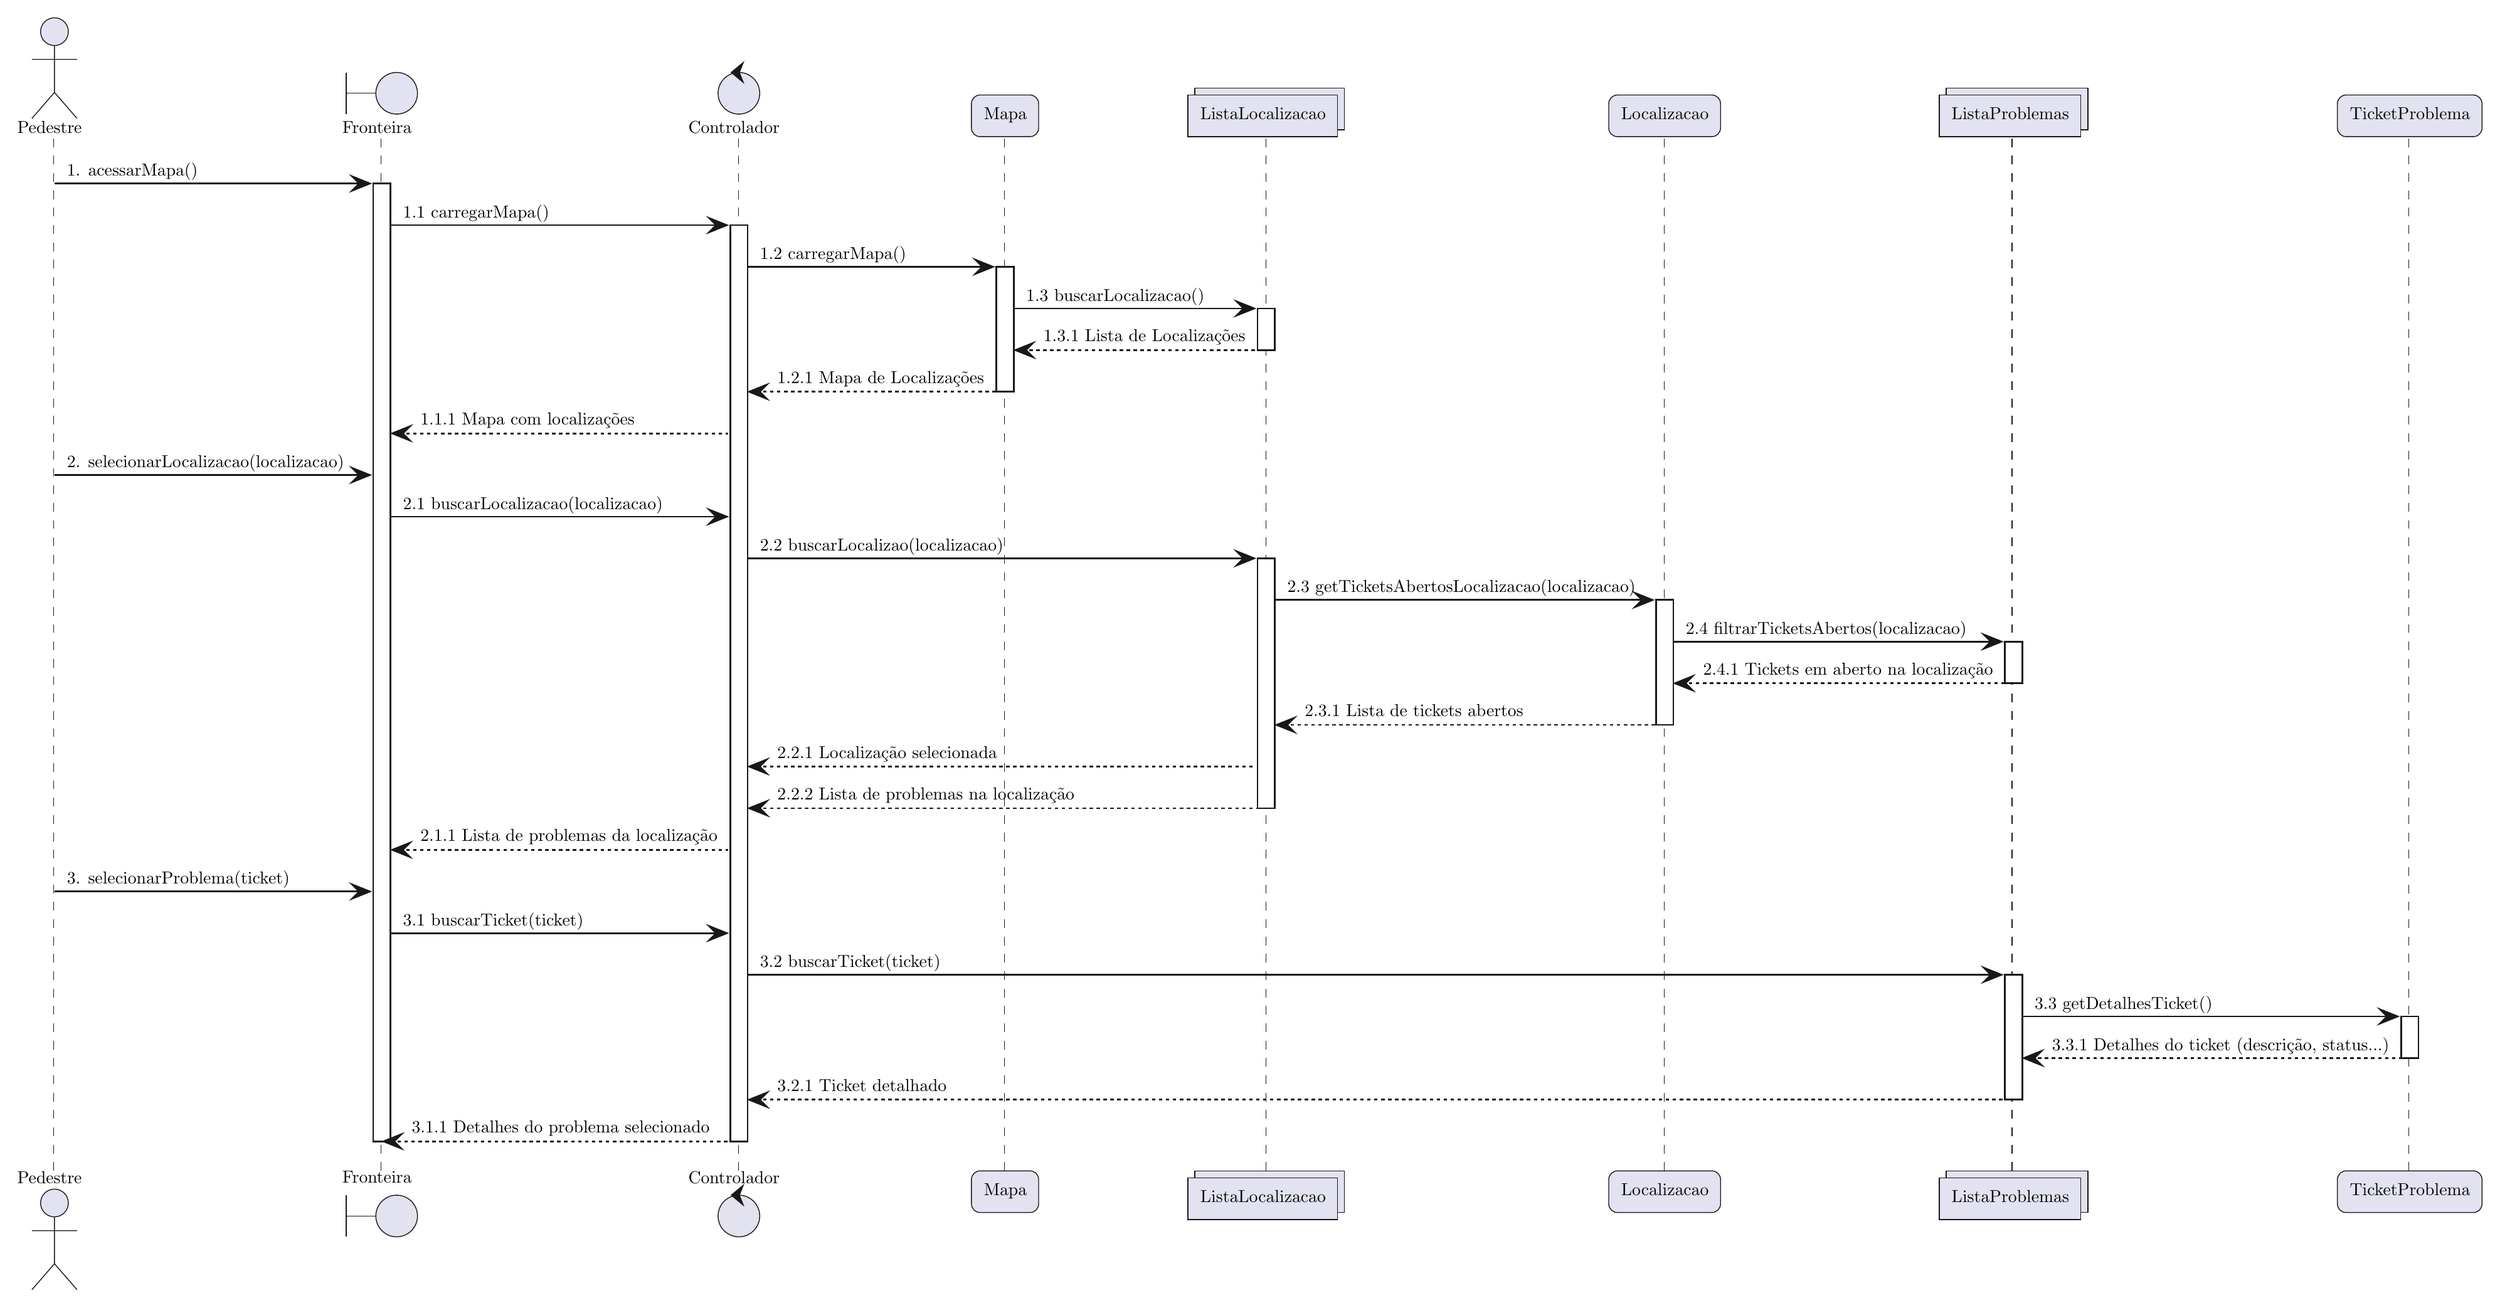
\begin{tikzpicture}[yscale=-1
,pstyle0/.style={color=plantucolor0001,fill=white,line width=1.0pt}
,pstyle1/.style={color=plantucolor0002,line width=0.0pt}
,pstyle2/.style={color=plantucolor0001,line width=0.5pt,dash pattern=on 5.0pt off 5.0pt}
,pstyle3/.style={color=plantucolor0001,fill=plantucolor0004,line width=0.5pt}
,pstyle4/.style={color=plantucolor0001,line width=0.5pt}
,pstyle5/.style={color=plantucolor0001,fill=plantucolor0001,line width=1.0pt}
,pstyle6/.style={color=plantucolor0001,line width=1.0pt}
,pstyle7/.style={color=plantucolor0001,line width=1.0pt,dash pattern=on 2.0pt off 2.0pt}
]
\draw[pstyle0] (210.23pt,101pt) rectangle (220.23pt,653pt);
\draw[pstyle0] (415.89pt,125pt) rectangle (425.89pt,653pt);
\draw[pstyle0] (569.24pt,149pt) rectangle (579.24pt,221pt);
\draw[pstyle0] (719.72pt,173pt) rectangle (729.72pt,197pt);
\draw[pstyle0] (719.72pt,317pt) rectangle (729.72pt,461pt);
\draw[pstyle0] (949.25pt,341pt) rectangle (959.25pt,413pt);
\draw[pstyle0] (1150.25pt,365pt) rectangle (1160.25pt,389pt);
\draw[pstyle0] (1150.25pt,557pt) rectangle (1160.25pt,629pt);
\draw[pstyle0] (1378.51pt,581pt) rectangle (1388.51pt,605pt);
\draw[pstyle1] (22.58pt,75pt) rectangle (30.58pt,671pt);
\draw[pstyle2] (26pt,75pt) -- (26pt,671pt);
\draw[pstyle1] (211.23pt,75pt) rectangle (219.23pt,671pt);
\draw[pstyle2] (214.73pt,75pt) -- (214.73pt,671pt);
\draw[pstyle1] (416.89pt,75pt) rectangle (424.89pt,671pt);
\draw[pstyle2] (420.605pt,75pt) -- (420.605pt,671pt);
\draw[pstyle1] (570.24pt,75pt) rectangle (578.24pt,671pt);
\draw[pstyle2] (573.875pt,75pt) -- (573.875pt,671pt);
\draw[pstyle1] (720.72pt,75pt) rectangle (728.72pt,671pt);
\draw[pstyle2] (724.585pt,75pt) -- (724.585pt,671pt);
\draw[pstyle1] (950.25pt,75pt) rectangle (958.25pt,671pt);
\draw[pstyle2] (954.045pt,75pt) -- (954.045pt,671pt);
\draw[pstyle1] (1151.25pt,75pt) rectangle (1159.25pt,671pt);
\draw[pstyle2] (1154.43pt,75pt) -- (1154.43pt,671pt);
\draw[pstyle1] (1379.51pt,75pt) rectangle (1387.51pt,671pt);
\draw[pstyle2] (1382.845pt,75pt) -- (1382.845pt,671pt);
\node at (5pt,65pt)[below right,color=black,inner sep=0]{Pedestre};
\draw[pstyle3] (26.58pt,13.5pt) ellipse (8pt and 8pt);
\draw[pstyle4] (26.58pt,21.5pt) -- (26.58pt,48.5pt)(13.58pt,29.5pt) -- (39.58pt,29.5pt)(26.58pt,48.5pt) -- (13.58pt,63.5pt)(26.58pt,48.5pt) -- (39.58pt,63.5pt);
\node at (5pt,670pt)[below right,color=black,inner sep=0]{Pedestre};
\draw[pstyle3] (26.58pt,688.5pt) ellipse (8pt and 8pt);
\draw[pstyle4] (26.58pt,696.5pt) -- (26.58pt,723.5pt)(13.58pt,704.5pt) -- (39.58pt,704.5pt)(26.58pt,723.5pt) -- (13.58pt,738.5pt)(26.58pt,723.5pt) -- (39.58pt,738.5pt);
\node at (192.265pt,65pt)[below right,color=black,inner sep=0]{Fronteira};
\draw[pstyle4] (194.73pt,37pt) -- (194.73pt,61pt)(194.73pt,49pt) -- (211.73pt,49pt);
\draw[pstyle3] (223.73pt,49pt) ellipse (12pt and 12pt);
\node at (192.265pt,670pt)[below right,color=black,inner sep=0]{Fronteira};
\draw[pstyle4] (194.73pt,684pt) -- (194.73pt,708pt)(194.73pt,696pt) -- (211.73pt,696pt);
\draw[pstyle3] (223.73pt,696pt) ellipse (12pt and 12pt);
\node at (391.605pt,65pt)[below right,color=black,inner sep=0]{Controlador};
\draw[pstyle3] (420.89pt,49pt) ellipse (12pt and 12pt);
\draw[pstyle5] (416.89pt,37pt) -- (422.89pt,32pt) -- (420.89pt,37pt) -- (422.89pt,42pt) -- (416.89pt,37pt) -- cycle;
\node at (391.605pt,670pt)[below right,color=black,inner sep=0]{Controlador};
\draw[pstyle3] (420.89pt,696pt) ellipse (12pt and 12pt);
\draw[pstyle5] (416.89pt,684pt) -- (422.89pt,679pt) -- (420.89pt,684pt) -- (422.89pt,689pt) -- (416.89pt,684pt) -- cycle;
\draw[pstyle3] (554.875pt,55pt) arc (180:270:5pt) -- (559.875pt,50pt) -- (588.605pt,50pt) arc (270:360:5pt) -- (593.605pt,55pt) -- (593.605pt,69pt) arc (0:90:5pt) -- (588.605pt,74pt) -- (559.875pt,74pt) arc (90:180:5pt) -- (554.875pt,69pt) -- cycle;
\node at (561.875pt,57pt)[below right,color=black,inner sep=0]{Mapa};
\draw[pstyle3] (554.875pt,675pt) arc (180:270:5pt) -- (559.875pt,670pt) -- (588.605pt,670pt) arc (270:360:5pt) -- (593.605pt,675pt) -- (593.605pt,689pt) arc (0:90:5pt) -- (588.605pt,694pt) -- (559.875pt,694pt) arc (90:180:5pt) -- (554.875pt,689pt) -- cycle;
\node at (561.875pt,677pt)[below right,color=black,inner sep=0]{Mapa};
\draw[pstyle3] (683.585pt,46pt) rectangle (769.855pt,70pt);
\draw[pstyle3] (679.585pt,50pt) rectangle (765.855pt,74pt);
\node at (686.585pt,57pt)[below right,color=black,inner sep=0]{ListaLocalizacao};
\draw[pstyle3] (683.585pt,670pt) rectangle (769.855pt,694pt);
\draw[pstyle3] (679.585pt,674pt) rectangle (765.855pt,698pt);
\node at (686.585pt,681pt)[below right,color=black,inner sep=0]{ListaLocalizacao};
\draw[pstyle3] (922.045pt,55pt) arc (180:270:5pt) -- (927.045pt,50pt) -- (981.455pt,50pt) arc (270:360:5pt) -- (986.455pt,55pt) -- (986.455pt,69pt) arc (0:90:5pt) -- (981.455pt,74pt) -- (927.045pt,74pt) arc (90:180:5pt) -- (922.045pt,69pt) -- cycle;
\node at (929.045pt,57pt)[below right,color=black,inner sep=0]{Localizacao};
\draw[pstyle3] (922.045pt,675pt) arc (180:270:5pt) -- (927.045pt,670pt) -- (981.455pt,670pt) arc (270:360:5pt) -- (986.455pt,675pt) -- (986.455pt,689pt) arc (0:90:5pt) -- (981.455pt,694pt) -- (927.045pt,694pt) arc (90:180:5pt) -- (922.045pt,689pt) -- cycle;
\node at (929.045pt,677pt)[below right,color=black,inner sep=0]{Localizacao};
\draw[pstyle3] (1116.43pt,46pt) rectangle (1198.07pt,70pt);
\draw[pstyle3] (1112.43pt,50pt) rectangle (1194.07pt,74pt);
\node at (1119.43pt,57pt)[below right,color=black,inner sep=0]{ListaProblemas};
\draw[pstyle3] (1116.43pt,670pt) rectangle (1198.07pt,694pt);
\draw[pstyle3] (1112.43pt,674pt) rectangle (1194.07pt,698pt);
\node at (1119.43pt,681pt)[below right,color=black,inner sep=0]{ListaProblemas};
\draw[pstyle3] (1341.845pt,55pt) arc (180:270:5pt) -- (1346.845pt,50pt) -- (1420.175pt,50pt) arc (270:360:5pt) -- (1425.175pt,55pt) -- (1425.175pt,69pt) arc (0:90:5pt) -- (1420.175pt,74pt) -- (1346.845pt,74pt) arc (90:180:5pt) -- (1341.845pt,69pt) -- cycle;
\node at (1348.845pt,57pt)[below right,color=black,inner sep=0]{TicketProblema};
\draw[pstyle3] (1341.845pt,675pt) arc (180:270:5pt) -- (1346.845pt,670pt) -- (1420.175pt,670pt) arc (270:360:5pt) -- (1425.175pt,675pt) -- (1425.175pt,689pt) arc (0:90:5pt) -- (1420.175pt,694pt) -- (1346.845pt,694pt) arc (90:180:5pt) -- (1341.845pt,689pt) -- cycle;
\node at (1348.845pt,677pt)[below right,color=black,inner sep=0]{TicketProblema};
\draw[pstyle0] (210.23pt,101pt) rectangle (220.23pt,653pt);
\draw[pstyle0] (415.89pt,125pt) rectangle (425.89pt,653pt);
\draw[pstyle0] (569.24pt,149pt) rectangle (579.24pt,221pt);
\draw[pstyle0] (719.72pt,173pt) rectangle (729.72pt,197pt);
\draw[pstyle0] (719.72pt,317pt) rectangle (729.72pt,461pt);
\draw[pstyle0] (949.25pt,341pt) rectangle (959.25pt,413pt);
\draw[pstyle0] (1150.25pt,365pt) rectangle (1160.25pt,389pt);
\draw[pstyle0] (1150.25pt,557pt) rectangle (1160.25pt,629pt);
\draw[pstyle0] (1378.51pt,581pt) rectangle (1388.51pt,605pt);
\draw[pstyle5] (198.23pt,97pt) -- (208.23pt,101pt) -- (198.23pt,105pt) -- (202.23pt,101pt) -- cycle;
\draw[pstyle6] (26.58pt,101pt) -- (204.23pt,101pt);
\node at (33.58pt,89pt)[below right,color=black,inner sep=0]{1. acessarMapa()};
\draw[pstyle5] (403.89pt,121pt) -- (413.89pt,125pt) -- (403.89pt,129pt) -- (407.89pt,125pt) -- cycle;
\draw[pstyle6] (220.23pt,125pt) -- (409.89pt,125pt);
\node at (227.23pt,113pt)[below right,color=black,inner sep=0]{1.1 carregarMapa()};
\draw[pstyle5] (557.24pt,145pt) -- (567.24pt,149pt) -- (557.24pt,153pt) -- (561.24pt,149pt) -- cycle;
\draw[pstyle6] (425.89pt,149pt) -- (563.24pt,149pt);
\node at (432.89pt,137pt)[below right,color=black,inner sep=0]{1.2 carregarMapa()};
\draw[pstyle5] (707.72pt,169pt) -- (717.72pt,173pt) -- (707.72pt,177pt) -- (711.72pt,173pt) -- cycle;
\draw[pstyle6] (579.24pt,173pt) -- (713.72pt,173pt);
\node at (586.24pt,161pt)[below right,color=black,inner sep=0]{1.3 buscarLocalizacao()};
\draw[pstyle5] (590.24pt,193pt) -- (580.24pt,197pt) -- (590.24pt,201pt) -- (586.24pt,197pt) -- cycle;
\draw[pstyle7] (584.24pt,197pt) -- (723.72pt,197pt);
\node at (596.24pt,185pt)[below right,color=black,inner sep=0]{1.3.1 Lista de Localizações};
\draw[pstyle5] (436.89pt,217pt) -- (426.89pt,221pt) -- (436.89pt,225pt) -- (432.89pt,221pt) -- cycle;
\draw[pstyle7] (430.89pt,221pt) -- (573.24pt,221pt);
\node at (442.89pt,209pt)[below right,color=black,inner sep=0]{1.2.1 Mapa de Localizações};
\draw[pstyle5] (231.23pt,241pt) -- (221.23pt,245pt) -- (231.23pt,249pt) -- (227.23pt,245pt) -- cycle;
\draw[pstyle7] (225.23pt,245pt) -- (414.89pt,245pt);
\node at (237.23pt,233pt)[below right,color=black,inner sep=0]{1.1.1 Mapa com localizações};
\draw[pstyle5] (198.23pt,265pt) -- (208.23pt,269pt) -- (198.23pt,273pt) -- (202.23pt,269pt) -- cycle;
\draw[pstyle6] (26.58pt,269pt) -- (204.23pt,269pt);
\node at (33.58pt,257pt)[below right,color=black,inner sep=0]{2. selecionarLocalizacao(localizacao)};
\draw[pstyle5] (403.89pt,289pt) -- (413.89pt,293pt) -- (403.89pt,297pt) -- (407.89pt,293pt) -- cycle;
\draw[pstyle6] (220.23pt,293pt) -- (409.89pt,293pt);
\node at (227.23pt,281pt)[below right,color=black,inner sep=0]{2.1 buscarLocalizacao(localizacao)};
\draw[pstyle5] (707.72pt,313pt) -- (717.72pt,317pt) -- (707.72pt,321pt) -- (711.72pt,317pt) -- cycle;
\draw[pstyle6] (425.89pt,317pt) -- (713.72pt,317pt);
\node at (432.89pt,305pt)[below right,color=black,inner sep=0]{2.2 buscarLocalizao(localizacao)};
\draw[pstyle5] (937.25pt,337pt) -- (947.25pt,341pt) -- (937.25pt,345pt) -- (941.25pt,341pt) -- cycle;
\draw[pstyle6] (729.72pt,341pt) -- (943.25pt,341pt);
\node at (736.72pt,329pt)[below right,color=black,inner sep=0]{2.3 getTicketsAbertosLocalizacao(localizacao)};
\draw[pstyle5] (1138.25pt,361pt) -- (1148.25pt,365pt) -- (1138.25pt,369pt) -- (1142.25pt,365pt) -- cycle;
\draw[pstyle6] (959.25pt,365pt) -- (1144.25pt,365pt);
\node at (966.25pt,353pt)[below right,color=black,inner sep=0]{2.4 filtrarTicketsAbertos(localizacao)};
\draw[pstyle5] (970.25pt,385pt) -- (960.25pt,389pt) -- (970.25pt,393pt) -- (966.25pt,389pt) -- cycle;
\draw[pstyle7] (964.25pt,389pt) -- (1154.25pt,389pt);
\node at (976.25pt,377pt)[below right,color=black,inner sep=0]{2.4.1 Tickets em aberto na localização};
\draw[pstyle5] (740.72pt,409pt) -- (730.72pt,413pt) -- (740.72pt,417pt) -- (736.72pt,413pt) -- cycle;
\draw[pstyle7] (734.72pt,413pt) -- (953.25pt,413pt);
\node at (746.72pt,401pt)[below right,color=black,inner sep=0]{2.3.1 Lista de tickets abertos};
\draw[pstyle5] (436.89pt,433pt) -- (426.89pt,437pt) -- (436.89pt,441pt) -- (432.89pt,437pt) -- cycle;
\draw[pstyle7] (430.89pt,437pt) -- (718.72pt,437pt);
\node at (442.89pt,425pt)[below right,color=black,inner sep=0]{2.2.1 Localização selecionada};
\draw[pstyle5] (436.89pt,457pt) -- (426.89pt,461pt) -- (436.89pt,465pt) -- (432.89pt,461pt) -- cycle;
\draw[pstyle7] (430.89pt,461pt) -- (723.72pt,461pt);
\node at (442.89pt,449pt)[below right,color=black,inner sep=0]{2.2.2 Lista de problemas na localização};
\draw[pstyle5] (231.23pt,481pt) -- (221.23pt,485pt) -- (231.23pt,489pt) -- (227.23pt,485pt) -- cycle;
\draw[pstyle7] (225.23pt,485pt) -- (414.89pt,485pt);
\node at (237.23pt,473pt)[below right,color=black,inner sep=0]{2.1.1 Lista de problemas da localização};
\draw[pstyle5] (198.23pt,505pt) -- (208.23pt,509pt) -- (198.23pt,513pt) -- (202.23pt,509pt) -- cycle;
\draw[pstyle6] (26.58pt,509pt) -- (204.23pt,509pt);
\node at (33.58pt,497pt)[below right,color=black,inner sep=0]{3. selecionarProblema(ticket)};
\draw[pstyle5] (403.89pt,529pt) -- (413.89pt,533pt) -- (403.89pt,537pt) -- (407.89pt,533pt) -- cycle;
\draw[pstyle6] (220.23pt,533pt) -- (409.89pt,533pt);
\node at (227.23pt,521pt)[below right,color=black,inner sep=0]{3.1 buscarTicket(ticket)};
\draw[pstyle5] (1138.25pt,553pt) -- (1148.25pt,557pt) -- (1138.25pt,561pt) -- (1142.25pt,557pt) -- cycle;
\draw[pstyle6] (425.89pt,557pt) -- (1144.25pt,557pt);
\node at (432.89pt,545pt)[below right,color=black,inner sep=0]{3.2 buscarTicket(ticket)};
\draw[pstyle5] (1366.51pt,577pt) -- (1376.51pt,581pt) -- (1366.51pt,585pt) -- (1370.51pt,581pt) -- cycle;
\draw[pstyle6] (1160.25pt,581pt) -- (1372.51pt,581pt);
\node at (1167.25pt,569pt)[below right,color=black,inner sep=0]{3.3 getDetalhesTicket()};
\draw[pstyle5] (1171.25pt,601pt) -- (1161.25pt,605pt) -- (1171.25pt,609pt) -- (1167.25pt,605pt) -- cycle;
\draw[pstyle7] (1165.25pt,605pt) -- (1382.51pt,605pt);
\node at (1177.25pt,593pt)[below right,color=black,inner sep=0]{3.3.1 Detalhes do ticket (descrição, status...)};
\draw[pstyle5] (436.89pt,625pt) -- (426.89pt,629pt) -- (436.89pt,633pt) -- (432.89pt,629pt) -- cycle;
\draw[pstyle7] (430.89pt,629pt) -- (1154.25pt,629pt);
\node at (442.89pt,617pt)[below right,color=black,inner sep=0]{3.2.1 Ticket detalhado};
\draw[pstyle5] (226.23pt,649pt) -- (216.23pt,653pt) -- (226.23pt,657pt) -- (222.23pt,653pt) -- cycle;
\draw[pstyle7] (220.23pt,653pt) -- (419.89pt,653pt);
\node at (232.23pt,641pt)[below right,color=black,inner sep=0]{3.1.1 Detalhes do problema selecionado};
\end{tikzpicture}
